\documentclass[11pt,letter]{article}

\usepackage[utf8x]{inputenc} %Unicode chars; æ,ø,å osv. 
%\usepackage[danish]{babel} %Danish LaTeX format; Chapters etc.
\usepackage{amsmath, amsfonts, amssymb} %Math symboler
\usepackage{ucs} %Greek letters
\usepackage{amsthm} %Custom environments
\usepackage{graphicx} %For figures
\usepackage[bookmarks=true,bookmarksopen=true,bookmarksnumbered=true]{hyperref} %Hyperrefs in PDF
\usepackage{url} %Handles URLs
%\usepackage{natbib} %bibliography package
%\usepackage[section]{placeins} %Package places a FloatBarrier before every section
\usepackage[top=1in,bottom=1in,left=1in,right=1in]{geometry} %Larger margins
\usepackage[usenames, dvipsnames]{xcolor} %Custom colors
\usepackage{tikz} %For tikz figures
%\usepackage{subfigure} %For subfigures
\usepackage{listings} %For code listings
\usepackage{textcomp} %Allows extra special symbols
\usepackage{algorithm} %For algorithms
\usepackage{cleveref} %Cref for all environment
\usepackage{pgfplots}
\usepackage{filecontents}

%Tikz stuff
\usetikzlibrary{shapes,arrows}  
\tikzstyle{block} = [rectangle, draw, text centered, rounded corners, minimum height=1cm]
\tikzstyle{line} = [draw, -latex']

%Bibliographystyle
\bibliographystyle{plain}

%Figure path
\graphicspath{{./Figures/}}

%Table of contents:
%
% - JavaScript

\definecolor{lightgray}{rgb}{.9,.9,.9}
\definecolor{dkgreen}{rgb}{0,0.6,0} %For comments in PHP

% % % % % % % % % % % % %  JAVASCRIPT % % % % % % % % % % % % % %
%Defines the JS in listings (not standard)
\definecolor{jsdarkgray}{rgb}{.4,.4,.4}
\definecolor{jspurple}{rgb}{0.65, 0.12, 0.82}

\lstdefinelanguage{JavaScript}{
  keywords={typeof, new, true, false, catch, function, return, null, catch, switch, var, if, in, while, do, else, case, break},
  keywordstyle=\color{blue}\bfseries,
  ndkeywords={class, export, boolean, throw, implements, import, this},
  ndkeywordstyle=\color{jsdarkgray}\bfseries,
  identifierstyle=\color{black},
  sensitive=false,
  comment=[l]{//},
  morecomment=[s]{/*}{*/},
  commentstyle=\color{jspurple}\ttfamily,
  stringstyle=\color{red}\ttfamily,
  morestring=[b]',
  morestring=[b]"
}
%Listings options
\lstset{ 
literate=%
{æ}{{\ae}}1
{å}{{\aa}}1
{ø}{{\o}}1
{Æ}{{\AE}}1
{Å}{{\AA}}1
{Ø}{{\O}}1,
  	basicstyle=\footnotesize, %Size of code
  	numbers=left, 
  	numberstyle=\tiny\color{black},
  	stepnumber=1,
 	backgroundcolor=\color{white},
    frame=single, % Frame style
    rulecolor=\color{black}, % Frame color
  	tabsize=4,
  	breaklines=true,
  	showstringspaces=false,
  	captionpos=b
}

%HEADER AND FOOTER
\usepackage{fancyhdr}
\fancyhf{}
\renewcommand{\footrulewidth}{\headrulewidth}
\fancyhead[LE]{\leftmark}
\fancyhead[OR]{\rightmark}
\fancyfoot[OR]{\thepage}
\fancyfoot[LE]{\thepage}
\author{Honam Bang and Jens Emil Gydesen}
\date{\today}
\title{Weekly Report - Week 9}
\begin{document}
\maketitle
\section{Project Summary}
We are developing a layer 7 load balancing system, codename ``Meercat'', that uses several load balancers to more efficiently balance the traffic amongst servers in a data center. The idea is that, rather than having a single load balancer, we have several load balancers that communicate with each other to load balance all servers. Each load balancer is able to send traffic to any server and we will use statistics to identify the required resources for each request.

We have looked at the Ananta (L4 software load balancer) paper (reference in the Duet paper from class)\cite{ananta} and also HAProxy\cite{haproxy}.

The goal is to, by having multiple load balancers, to more the system very scalable to a high amount of servers as well as eliminating having a single point of failure. 

\section{Progress}
In implementation part, We've implemented the multi load balancing system. Now we complete the implementation and we are on running several performance measurement. The features what we have implemented are:
\begin{enumerate}
	\item[a)] A Meercat communicate with all other n-1 Meercats to distribute traffic efficiently
	\item[b)]  A Meercat system consists of one master and multi slaves which are connected to each other.
	\item[c)]  A Meercat system takes advantages of multi loadbalancer system. When a master fails (power-off or error) while on running, one of the other slaves automatically takes over the role.
	\item[d)] A Meercat supports two routing algorithms; Round-Robin and CPU/MEM-usage-based routing. A master checks all CPU/MEM resource usage of hosts and propagates to slaves. All slaves ping to the master every seconds; if no response, the next slave becomes a master.
\end{enumerate}

The communication diagram between a master and slave are described in the below figure:
\begin{center}
	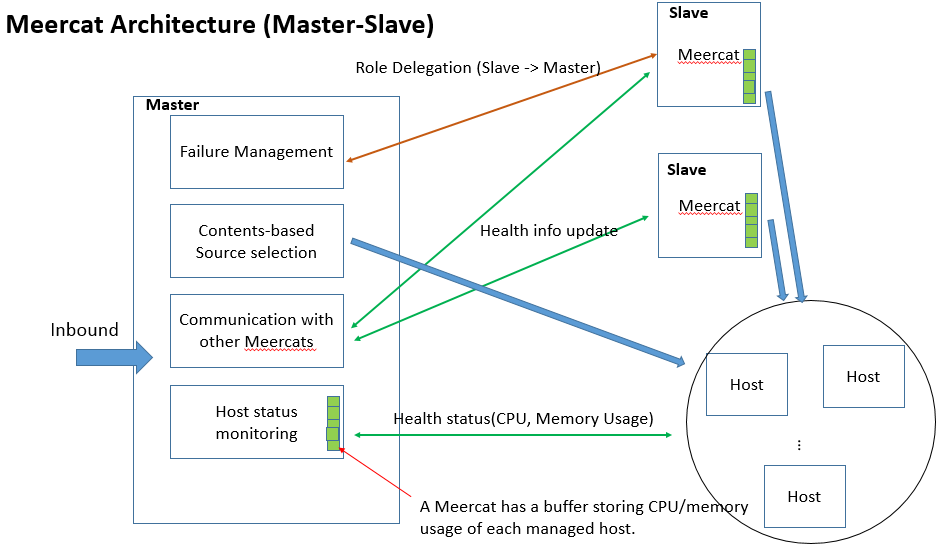
\includegraphics[scale=0.5]{./comm.png}
\end{center}

The only master can listen to resource status of hosts, and can propagates these information to slaves. All slaves ping to a master in every 1 sec. If a master get power-off or down, the next slave automatically takes over the master role (failover). A Meercat has three thread to handle multi channel communication as the below figure shows.
\begin{center}
	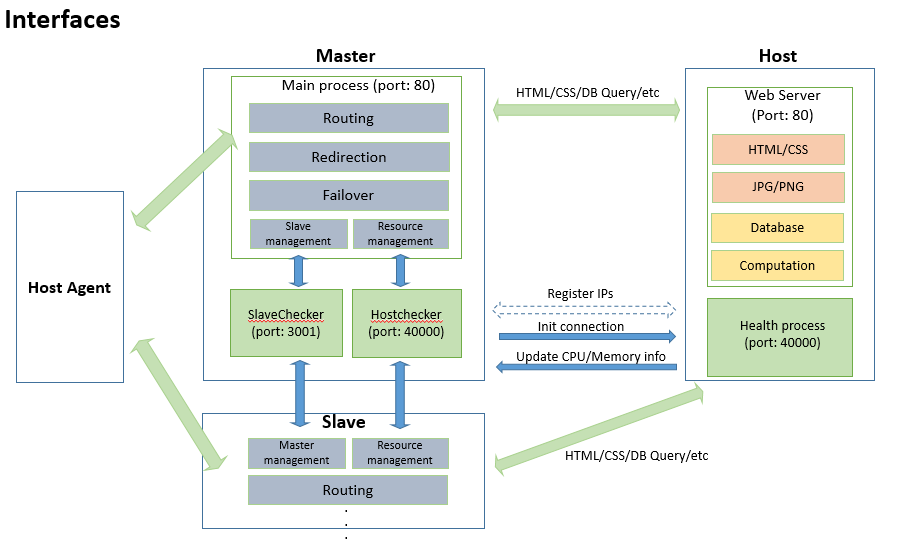
\includegraphics[scale=0.5]{./interface.png}
\end{center}

Our current results are not shown yet as the results from our tests showed that we need to optimize/fix the way the master gets information from the hosts. As of right now, this is not happening efficiently enough and a lot requests are sent to servers before we get information about their status.
 
\section{For Next Week}
For next week, we will improve the information gathering system and measure the performance of our Meercat. We will also prove whether our initial assumption-multi load balancer system would take advantages than a single load balancer in some specific area - is correct or wrong with several metrics. 

\begin{thebibliography}{9}
  \bibitem{ananta}
  Patel, Parveen, et al. "Ananta: Cloud scale load balancing." ACM SIGCOMM Computer Communication Review. Vol. 43. No. 4. ACM, 2013.
  \bibitem{haproxy}
  Tarreau, Willy. "HAProxy-The Reliable, High-Performance TCP/HTTP Load Balancer." 2011-8)[2013-4]. http://haproxy. lwt. eu (2012).
\end{thebibliography}
\end{document}
